\documentclass{article}

\usepackage{graphicx}
\usepackage{fullpage}
\usepackage{wrapfig}
\usepackage{float}
\usepackage{amsmath}


\graphicspath{ {img/} }

\usepackage{listings}
\usepackage{color}

\definecolor{dkgreen}{rgb}{0,0.6,0}
\definecolor{gray}{rgb}{0.5,0.5,0.5}
\definecolor{mauve}{rgb}{0.58,0,0.82}

\lstset{frame=tb,
  language=C++,
  aboveskip=3mm,
  belowskip=3mm,
  showstringspaces=false,
  columns=flexible,
  basicstyle={\small\ttfamily},
  numbers=none,
  numberstyle=\tiny\color{gray},
  keywordstyle=\color{blue},
  commentstyle=\color{dkgreen},
  stringstyle=\color{mauve},
  breaklines=true,
  breakatwhitespace=true,
  tabsize=3
}

\begin{document}

\title{Program 4 Design and Analysis}
\author{Julian Brackins, Ryan Feather, Joe Mowry and Charles Bonn}
\date{12/9/2014}
\maketitle

\section{Project Proposal}

We will be designing a protocol for paralellizing hash table operations.

We will have two solutions. One in a shared memory architecture where each worker thread has access to a shared hash table. And another on a distributed architecture that divides the hash table into segments, making each node responsible for operations of their own segment of the table.

In this directory, the shared memory solution is located in the "shared" directory, and the distributed memory solution is located in the "distributed" directory. Each solution has its own Makefile, source code, 
and corresponding doxygen documentation that can be generated by running "make dox" in the respective solution directory. The generated documentation can then be opened by running "make read" in the solution 
directory if Google Chrome has been installed.

\section{Libraries Used}

The shared memory solution was created using the The OpenMP API specification for parallel programming. The distributed memory solution 
was created using the Opem MPI message passaging interface library.

\section{Part 1 - Shared Memory}

\subsection{Program Description}

\subsection{Design}
Following Foster's design methodology, we have a brief overview:

\subsubsection{Partitioning}
        \begin{itemize}
            \item Reading values to be hashed
            
            In order to have the values hashed into the table, there must first be a list of values. In the shared memory test, 
            an array is utilized to generate a list of random strings to be inserted into the hash table. This initialization of 
            the list must occur first in the program in order to have the list available for the three tests: the serial runtime, 
            the parallel runtime using static scheduling, and the parallel runtime using dynamic scheduling.
            \item Hashing
            
            The following code overviews the actual Hashing method used in this program. the hash key is multiplied by 31 by 
            shifting the previous hash value by 5, which is equivalent to multiplying by 2 to the 5th, then subtracting the hash value. 
            This hash value is then modded by the Hash table size to place the hash key within range of the table indices.
            \begin{lstlisting}
unsigned int HashTable::Hash(std::string str)
{
  unsigned int hashval;

  /// initialize hash to 0
  hashval = 0;
  char* t = const_cast<char*>(str.c_str());

  /// Multiply old hash value by 31.
  /// hashval << 5 = multiplying by 2^5 (32) minus hashval = 31.
  /// Shifts are faster than multiplication while still doing what we
  /// want to do. 
  for(; *t != '\0'; t++)
    hashval = *t + (hashval << 5) - hashval;

  /// mod the hash value by the table size so it fits in the range.
  return hashval % GetTableSize();
}
	    \end{lstlisting}
            
            \item Sending and Recieving
            
            Sending and Receiving are fairly trivial tasks in the omp implementation for the parallelization of this hash table.
            \item Inserting
            
            Inserting into the table will have interesting data dependency. In this implementation, we have assumed that no two 
            strings being inserted into the table will be alike. In a real life situation, for instance, values would be hashed into 
            a table using a unique hash key, or ID. That is to say, with a hash table that holds student records, each student would 
            be inserted into the hash using their student ID as their hash key. Therefore, duplicate data would not be added into a 
            hash table. 
            
            Since we operate on this assumption that multiple values will not occupy a given index of the hash table, no node of the 
            hash table will be accessed by more than one task at any given time.
        \end{itemize}
\subsubsection{Communication}
        \begin{itemize}
            \item Sharing data between computations
            
            Previously stated, the act of sharing between tasks is somewhat minimal. Each task will be handling different nodes of the 
            hash table, so there is no issue of accessing and writing to the same node at a given point during the insertion phase. 
            However, there is an issue of updating the total number of entries into the hash table. This is handled by placing a 
            critical block around the two functions that handle the incrementation and decrementation of the table count, as seen here: 
	    \begin{lstlisting}
void HashTable::IncTableCount()
{
# pragma omp critical(dataupdate)
  table_count++;
}

void HashTable::DecTableCount()
{
# pragma omp critical(dataupdate)
  table_count--;
}
	    \end{lstlisting}
	    
            \item Determine amount and pattern of communication
            
            Therefore, the amount of communication is determined. The only global communication among the tasks is to handle the updating of 
            the table size.
        \end{itemize}
\subsubsection{Aglomeration}
        \begin{itemize}
            \item Combine or group tasks to improve performance
            
            This section will analyze the tasks identified during the Partitioning section to determine how tasks can be grouped together: 
            
             \begin{itemize}
		\item Reading values to be hashed
		\item Hashing
		\item Inserting
		\item Update Table Count
	    \end{itemize}
		
		Generating the values to be hashed needs to be done as its own task, in order to have the list of values to hash 
		be the identical for each of the three runs.

		Hashing and Inserting to the table can be combined into the same task. A hash key is generated based on the string 
		being inserted into the table, and then the value is inserted into the table. By combining these two tasks, the 
		entire loop of iterating through the values to be hashed can be parallelized. Updating Table Count is also grouped 
		into this task block, as it needs to be done after every succesful insert.
        \end{itemize}
\subsubsection{Mapping}
        \begin{itemize}
            \item Assign agglomerated tasks to threads/physical processors.
            
            The following code block details the three different tests and how the threads are mapped to the tasks. As stated, the 
            shared memory solution for OMP is more or less trivial when it comes to mapping. The for loop is parallelized for the 
            list of strings to be added to the hash, with each thread performing a chunk of the strings at a time. The data isn't 
            sequential in any way, so the order of the strings being inserted should not be an issue.
	    \begin{lstlisting}
  ///Run and time the Serial solution
  start = omp_get_wtime( );
# pragma omp parallel for schedule(dynamic, 1) num_threads(1)
  for( i = 0; i < list_size; i++)
    ht1->AddString(strList[i]);
  finish = omp_get_wtime();
  serial_t = timeOMP(start, finish);

  ///Run and time the Parallel (Static) solution
  start = omp_get_wtime();
# pragma omp parallel for schedule(static, chunk_size) num_threads(thread_count)
  for( i = 0; i < list_size; i++)
    ht2->AddString(strList[i]);
  finish = omp_get_wtime();
  static_t = timeOMP(start, finish);

  ///Run and time the Parallel (Dynamic) solution
  start = omp_get_wtime( );
# pragma omp parallel for schedule(dynamic, chunk_size) num_threads(thread_count) 
  for( i = 0; i < list_size; i++)
    ht3->AddString(strList[i]);
  finish = omp_get_wtime( );
  dynamic_t = timeOMP(start, finish);
	    \end{lstlisting}
        \end{itemize}


\subsection{Performance Testing}
The following figures overview the timing analysis for the shared memory solution for our hash table.
The raw data can be found in the timing analysis excel file in the documentation directory of
our project.
\begin{figure}[H]
  \caption{Timing Evaluation of increasing problem size}
  \centering
  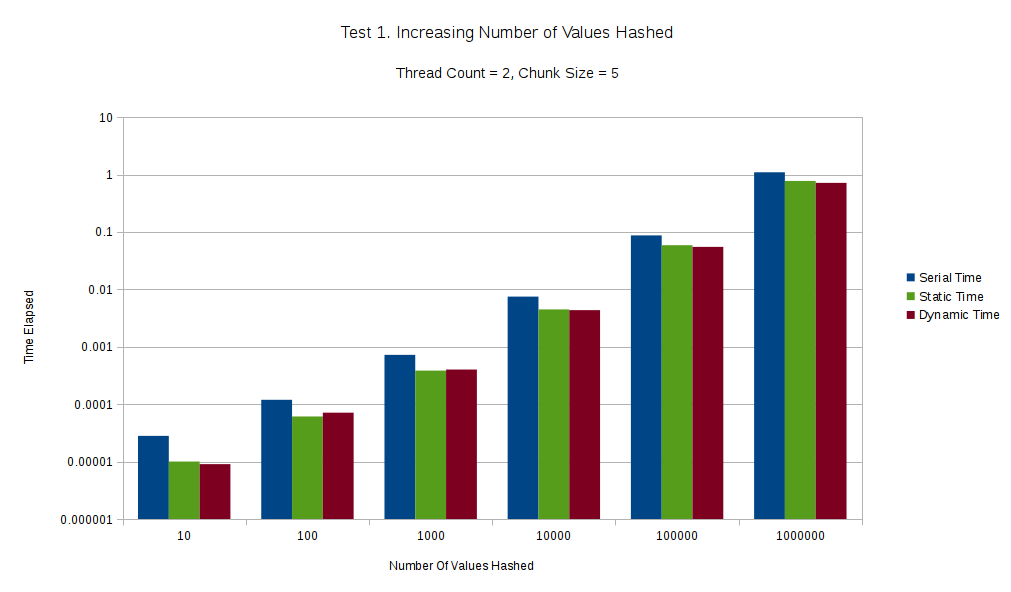
\includegraphics[width=\textwidth]{chart1a}
  \label{fig:chart1a}
\end{figure}

Figure~\ref{fig:chart1a} displays the timing evaluation of the shared memory hash table as the problem 
size is scaled up. In each run, the number of values added to the hash table are increased by a factor 
of 10. The strings added to the hash table are randomized, and every string is unique, since identical 
strings cannot be added to this hash table. As the problem size increases, the parallel solutions complete 
the tasks of inserting into the table faster than the serial solution.

\begin{figure}[H]
  \caption{Speedup / Efficiency Evaluation of increasing problem size}
  \centering
  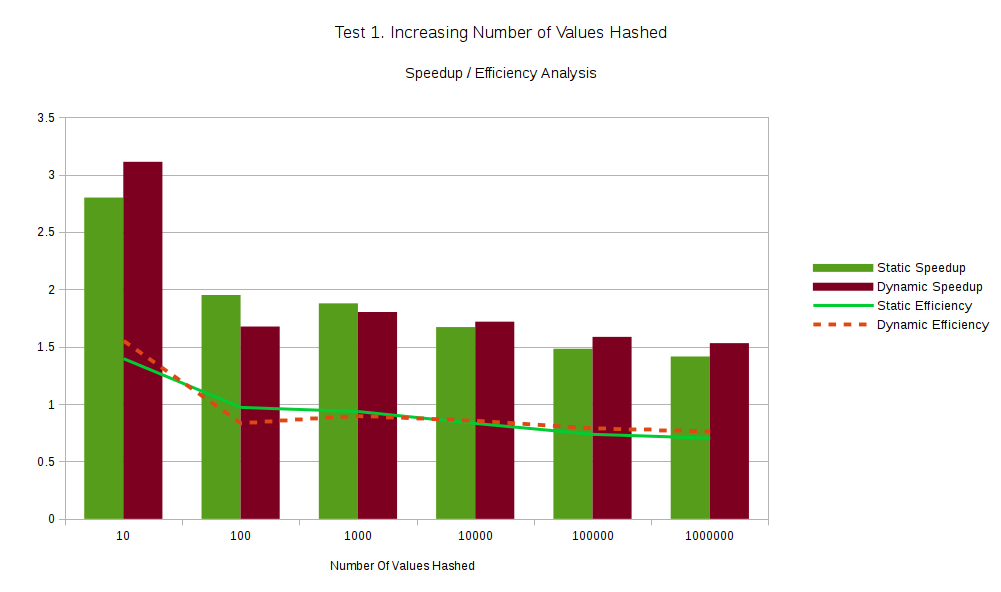
\includegraphics[width=\textwidth]{chart1b}
  \label{fig:chart1b}
\end{figure}

Figure~\ref{fig:chart1b} is the analysis of the speedup and efficiency gained by using the parallel solutions, 
both static and dynamic scheduling, on an increasing problem size. While we did observe in Figure~\ref{fig:chart1a} 
that the two parallel solutions were consistently faster than the serial counterpart, the actual speedup and 
efficiency observed as the problem size increases has a downward trend. Therefore, we can conclude that as the 
problem size increases, the speedup and efficiency of the parallel solution decreases, despite an overall better 
time performance.

\begin{figure}[H]
  \caption{Timing Evaluation of increasing thread count}
  \centering
  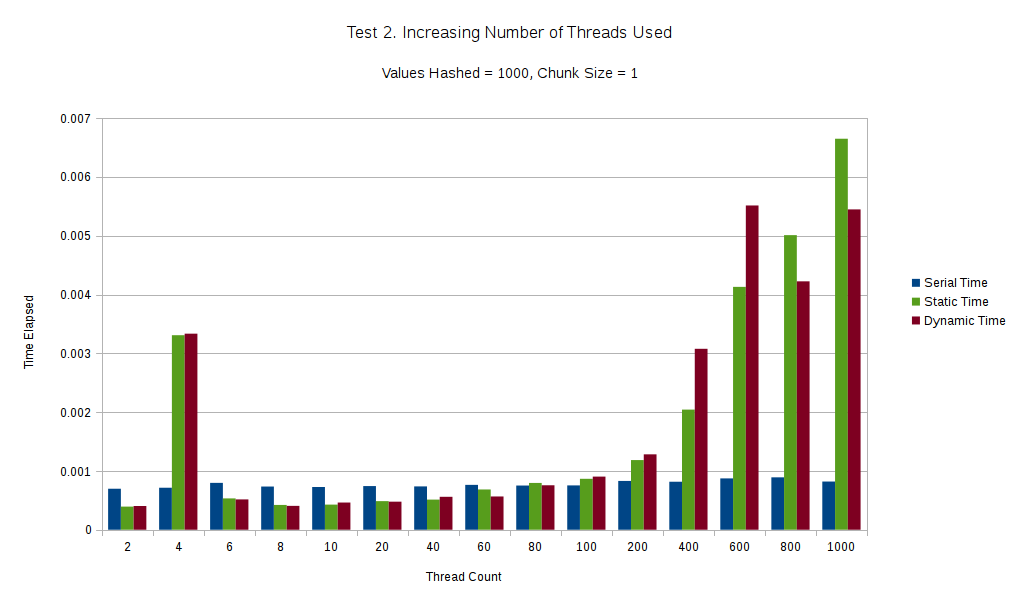
\includegraphics[width=\textwidth]{chart2a}
    \label{fig:chart2a}
\end{figure}

Figure~\ref{fig:chart2a} observes the timing evaluation of the shared memory hash table as the amount of threads 
increases. For smaller thread counts (2, 6 through around 60) the program overall has a better performance on the 
parallel versions as opposed to the serial method, but for larger thread counts (80+), the program actually 
performs better serially due to the amount of overhead from thread management. It should be noted that there is 
a rather peculiar spike in runtime for the parallel methods when running the program with 4 threads. For whatever 
reason, the program takes an incredibly long time when utilizing 4 threads, but returns to the expected trend 
with all other thread counts.

\begin{figure}[H]
  \caption{Speedup / Efficiency Evaluation of increasing thread count}
  \centering
  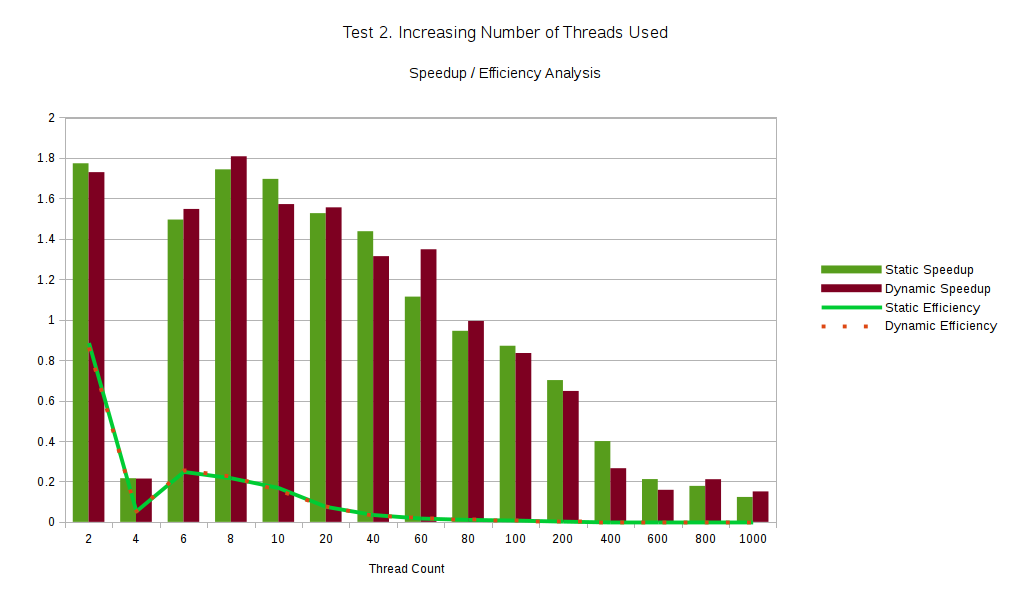
\includegraphics[width=\textwidth]{chart2b}
    \label{fig:chart2b}
\end{figure}

Figure~\ref{fig:chart2b} reflects this peculiar anomaly at a thread count of 4, but otherwise shows a mostly 
downward trend of both speedup and efficiency as more threads are used in the program. According to the chart, 
the Static scheduling method experiences the greatest speedup and efficiency at 2 threads. The Dynamic scheduling 
method, while technically having the greatest speedup rating at 8 threads, is most efficient at 2 threads as well.

\begin{figure}[H]
  \caption{Timing Evaluation of increasing chunk size}
  \centering
  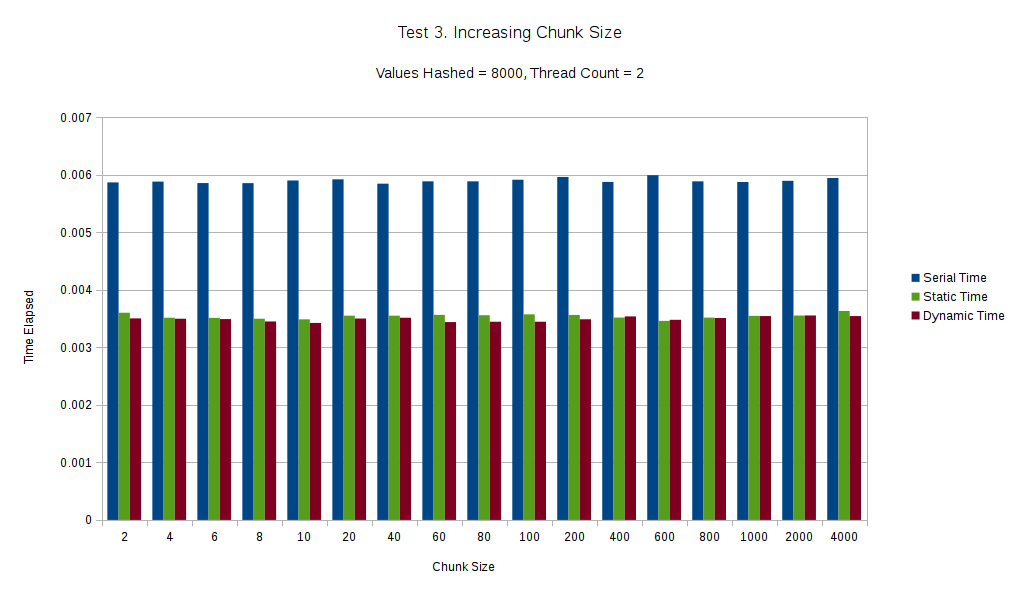
\includegraphics[width=\textwidth]{chart3a}
    \label{fig:chart3a}
\end{figure}

Figure~\ref{fig:chart3a} details the timings of the hash table inserts when the chunk size is increased on the 
parallel solutions. As this diagram illustrates, increasing chunk size has a somewhat noteworthy effect on the 
amount of time it takes for the program to run. Curiously, however, the amount of time required to run the program 
is basically identical over all tests as the chunk size increases. As long as the chunk size is greater than 1, the 
parallel solutions observe a faster runtime than the serial method, although this faster runtime is identical even 
as the chunk size increases.

\begin{figure}[H]
  \caption{Speedup / Efficiency Evaluation of increasing chunk size}
  \centering
  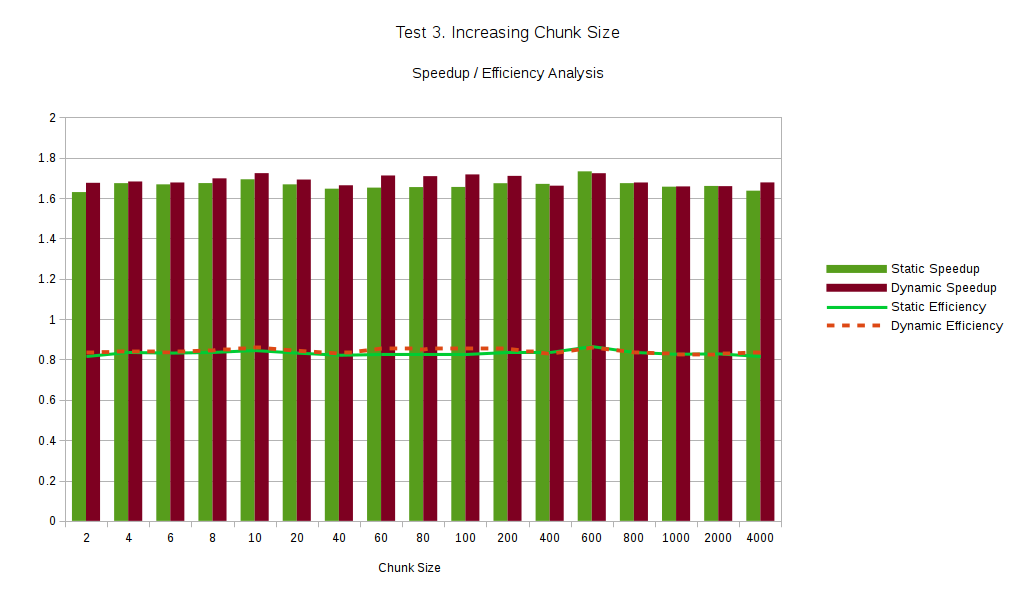
\includegraphics[width=\textwidth]{chart3b}
    \label{fig:chart3b}
\end{figure}

As a result of this observation, Figure~\ref{fig:chart3b} features a mostly horizontal trend in both speedup and efficiency as the chunk size given to each task increases in the parallel solution. 

\section{Part 2 - Distributed memory}
\subsection{Program Description}
This distributed memory program will allow for the typical hash table operations, but on a set of programs on potentially different computers.

Each process on each machine will be responsible for its own hash table, and respond to messages from a managing producer thread. The managing thread will give values to store and request table lookups.

The data is currently random strings read in from a file. A few sample inputs are provided.

\subsection{Design}
Following Foster's design methodology, we have a brief overview:

\subsubsection{Partitioning}
For our distributed memory solution, as in our shared, we will be doing data-centric partitioning. We will assign to each piece of data (in this case the strings) the tasks of hashing that data and storing it into a table. 

This will create a large number of tasks, much larger than our number of processors. There are no redundant computations, and each take will be roughly the same size.

\subsubsection{Communication}
For each piece of data, in order to place it in a table, it must first be hashed according to the hash function. This is an example of local communication. Therefore, since the tasks are dependent, we can consolidate them into one single task, hashing and storing a value.

In addition, the tasks associated with a piece of data will work very independently. Very little global communication will be needed.

Communication is balanced, minimized, and all tasks can be performed concurrently.

\subsubsection{Agglomeration}
As discussed in the last section, each piece of data can be consolidated into one combined operation.

Other than that, there is not much agglomeration that can be done. Because the work associated with each piece of data is independent of the solution as a whole, and the locality of the table insert is minimal, we cannot group together tasks in a meaningful or advantageous way.

\subsubsection{Mapping}
For the distributed memory solution, we will employ a producer-consumer structure. We will have one root thread that produces values from an input file, handing out the values to the consumer threads. Each consumer thread will take the piece of data, hash it, and place it in the table.

It is very important that we balance the load that each consumer thread experiences, making sure that they are not overwhelmed with data that will make computation take longer or potentially fill up their table. At the same time, we want to make sure that the storing of data is deterministic, that way we can find the data in a later lookup operation. In order to do this, the data is hashed twice. Once by the root producer thread in order to determine which worker thread will get the data, and again by the worker to determine where in its table to place the data.



\subsection{Performance Testing}
In order to test the performance of the implementation, timing data is recorded by the program. The program is given a set number of random strings that it must hash into tables. It is then given another set of values that it will attempt to lookup in the created hash tables.

As can be seen in Figure \ref{fig:dist_1}, increasing the problem size has a very direct correlation to the execution time.
\begin{figure}[H]
  \caption{Increasing Problem Size}
  \centering
  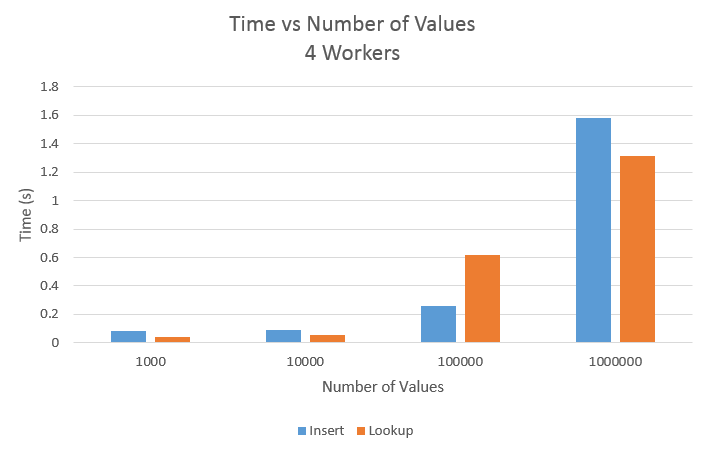
\includegraphics[width=\textwidth]{dist_1}
    \label{fig:dist_1}
\end{figure}
The results show are not surprising considering the nature of the algorithm. Increasing the number of values hashed and stored means an increase in the amount of communication and computation.

So how do these numbers look when applied to various sizes of the worker pool? As can be seen in Figure \ref{fig:dist_2}, we have a general increase in execution time as our worker pool increases. This unfortunately goes against the aims of the parallel implementation, as we would like to see an improvement in execution time. There are a few explanations for what causes this, but the leading cause is almost certainly the increase in communication as number of threads increases.

\begin{figure}[H]
  \caption{Time vs Number of Threads}
  \centering
  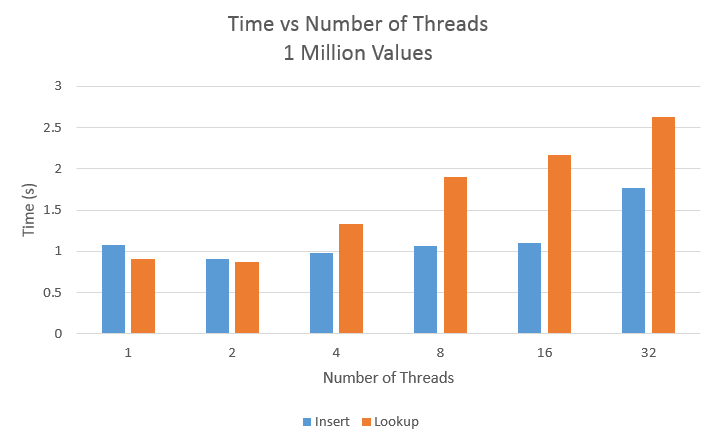
\includegraphics[width=\textwidth]{dist_2}
    \label{fig:dist_2}
\end{figure}

And as can be seen in our last figure, Figure \ref{fig:dist_3}, the efficiency of our parallelism becomes very small for large numbers of threads.
\begin{figure}[H]
  \caption{Speedup / Efficiency Evaluation for Number of Threads}
  \centering
  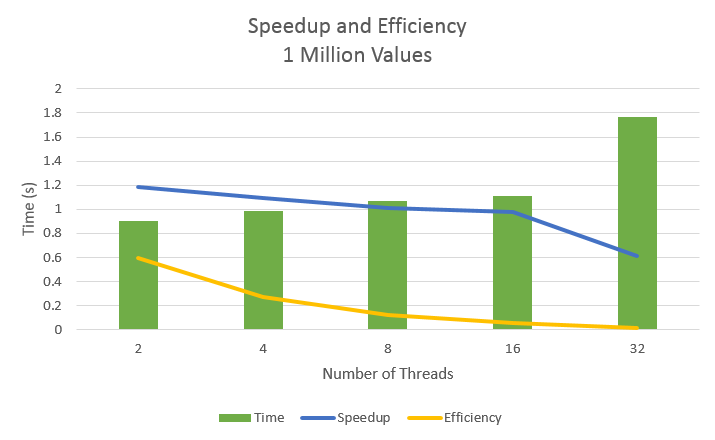
\includegraphics[width=\textwidth]{dist_3}
    \label{fig:dist_3}
\end{figure}


One improvement to the distributed implementation that might give better results would be to do communication from the root thread in batches. For example, only sending out values to a worker thread once the number of values ``sent'' is equal to some number. This would allow for less communication overall and reduce the amount of time that the root thread spends sending messages.


\section{Deliverables}
  The following is a list of items and directories located in this project submission:
  \begin{itemize}
	\item prog4 (directory):
	  \begin{itemize}
	    \item distributed (directory): Directory containing distributed method source code (src directory), headers (inc directory) and doxygen files (doc directory). Run "make" to build project, run "make dox" to build doxygen documentation, and run "make read" to open the html doxygen documentation in Google Chrome.

	    \item shared (directory): Directory containing shared method source code (src directory), headers (inc directory) and doxygen files (doc directory). Run "make" to build project, run "make dox" to build doxygen documentation, and run "make read" to open the html doxygen documentation in Google Chrome.
	    
	    \item genstr.py: python script used to generate random strings.
	  \end{itemize}
  \end{itemize}          

\end{document}
